\documentclass[10pt]{article}

% Language setting
% Replace `english' with e.g. `spanish' to change the document language
\usepackage[spanish]{babel}

% Set page size and margins
% Replace `letterpaper' with `a4paper' for UK/EU standard size
\usepackage[letterpaper,top=2cm,bottom=2cm,left=3cm,right=3cm,marginparwidth=1.75cm]{geometry}

% Useful packages
\usepackage{amsmath}
\usepackage{graphicx}
\usepackage[colorlinks=true, allcolors=blue]{hyperref}
\usepackage{authblk}
\usepackage[font=large,labelfont=bf]{caption}
\usepackage{float}
\usepackage{tikz}
\usepackage{amsfonts}
\usepackage{amsthm}
\usepackage{amsmath}
\usepackage{amssymb}
\usepackage{listings}
\usepackage{xcolor}
\usepackage{booktabs}
\usepackage{siunitx}
\usepackage{array}
\usepackage{dcolumn}
\usepackage{bbm}
\usepackage{subfig}
\usepackage{scrextend}
\usepackage{hyperref}
\usepackage{titlesec}
\usepackage{siunitx}

\geometry{
    left=1.5cm,
    right=1.5cm,
    top=1.5cm,
    bottom=1.5cm
}



\addto\captionsspanish{
\def\listtablename{\'Indice de tablas}%
\def\tablename{Tabla}}
\deffootnote[2em]{2em}{1em}{\textsuperscript{\thefootnotemark}\,}


\title{\textbf{Taller 3 Big Data \& Machine learning}}
\author{Hugo Sabogal, Gabriela Pérez, Maria Paula Osuna, Juan Andrés Silva}
\affil{Universidad de los Andes \\ Facultad de Economía}

\date{26 de mayo de 2024}



\begin{document}
\maketitle

\begin{center}
    \href{https://github.com/Hugo-Andres-Sabogal-Perez/Problem-set-3}{\label{repo}Repositorio de GitHub}
\end{center}

\section{Introducción}
En los últimos años, Colombia ha experimentado una significativa desaceleración en el sector inmobiliario, principalmente debido a la dependencia de las tasas de interés y los cambios en las políticas públicas. Esta situación ha llevado a una disminución notable en la actividad económica del sector vivienda (construcción), afectando los precios de las propiedades según la oferta y la demanda. Concretamente, el sector vivienda cayó 3.1 puntos porcentuales entre 2022 y 2023, aunque recientemente ha mostrado una recuperación con un aumento de 1.1 puntos porcentuales en el trimestre mas reciente del año 2024 (Dane, 2024). Ante este panorama, donde la actividad económica de la vivienda sufre grandes fluctuaciones en la oferta y la demanda, se vuelve crucial el uso de herramientas innovadoras como los modelos predictivos de machine learning. Estas herramientas pueden ayudar a identificar con precisión los precios del mercado mediante el análisis de características observables de las propiedades y el uso de algoritmos avanzados que permitan estimar con mayor exactitud el precio real de las mismas. \\

Adicionalmente, con el objetivo de evitar repetir el colapso significativo que tuvo el sector inmobiliario en Estados Unidos gracias al plan de inteligencia artificial Zillow y la sobreestimación de los precios de los bienes raíces que generó el mismo, el presente trabajo busca generar una serie de modelos de predicción que estime el precio hedónico de las viviendas específicamente en Bogotá, Colombia. Para esto, se tomaron diferentes amenidades y se buscó la mejor combinación para predecir la variable respuesta y lograr una buena predicción de ésta a partir de una base de datos consolidada. \\

Los datos que se utilizaron a lo largo de este ejercicio constaban de diferentes problemáticas que se tomaron en cuenta y solucionaron durante su desarrollo; entre estos se puede recalcar la mala construcción de variables como el área construida de las viviendas (dada la aparición de alta cantidad de outliers y missing values) y la recopilación de información sobre los atributos físicos de las viviendas a partir de la descripción de las variables. Adicionalmente, es importante recalcar que la base de datos consolidada contiene variables que se agregaron y construyeron a partir de fuentes externas como, por ejemplo, diferentes variables que calculan las distancias de los inmuebles a los sitios de mayor interés social.  \\

A partir de la estimación de los diferentes modelos, se llegó a la conclusión que la mejor estimación, con un MAE de 183’500,000 COP, se predijo a partir de un modelo de ensamble en el que se combinaron los dos mejores modelos de boosting resultantes, uno estimado a partir del algoritmo de lightgbm y otro utilizando extreme gradient boosting (xgb). A pesar de los buenos resultados de este modelo por fuera de muestra, es importante para futuras investigaciones tener en cuenta que aun así este se desfasa por 180 millones en promedio lo que impide tener confiabilidad en los modelos para valorar adecuadamente bienes inmuebles y de esta forma lograr identificar posibles oportunidades de negocio que permitan la compra de bienes inmuebles por debajo de su precio potencial.  

\section{Datos}

Para el presente trabajo, se utilizó una base de datos\footnote{Es importante tener claro que la base de datos se divide en dos, una de entrenamiento y otra de testeo.}  de propiedades en Bogotá tomada de la página web Properati\footnote{Se trata de una página web fundada en 2012 para venta y alquiler de inmuebles en 5 países de Latinoamérica entre los cuales se encuentra Colombia.}  con el objetivo de generar un modelo predictivo que haga posible la compra de la mayor cantidad de inmuebles en el barrio Chapinero al menor costo y evitando el fiasco de Zillow, el cual generó grandes pérdidas dado que sus datos no coincidían con los del mundo real, lo que llevó a la creación de un modelo erróneo que sobreestimaba el precio de los inmuebles. “Agentes inmobiliarios e inversores han afirmado durante mucho tiempo que los precios que figuran en Zillow tienden a ser más altos de lo que los compradores están dispuestos a pagar, lo que les da a los propietarios una idea distorsionada de lo que vale su casa” (Knauff, J. 2021). \\

Para cumplir con este objetivo y hacer uso adecuado de los datos proveídos inicialmente se debió realizar un exhaustivo análisis para la limpieza, organización y agregación de nuevas variables a la base de datos tanto de entrenamiento como de testeo. De esta manera se logró llegar a bases de datos limpias y únicamente con variables adecuadas para el desarrollo de los modelos de predicción. A continuación se encuentra la descripción detallada de este proceso. \\

Inicialmente, las bases de datos contenían 38,644 observaciones con 16 variables en el caso de la de entrenamiento y 10,286 observaciones con 16 variables para la de testeo. Adicional a estas, se crearon aproximadamente 60 nuevas variables tanto demográficas, de distancia como de seguridad ciudadana; para la construcción de estas variables fueron indispensables dos fuentes: la alcaldía de Bogotá y Open Street Map, pues a partir de estas se tomaron los datos para construir variables como por ejemplo la distancia a la estación de Transmilenio, a la parada de SITP, al centro comercial, al restaurante o gastro bar más cercana, etc. Es importante recalcar que la construcción de estas variables de distancia se logró a través de las variables de longitud y latitud y el cálculo lineal de ésta a partir del código en R Studio. Por el lado de las variables de delitos, dado que estas se encontraban a nivel localidad, se generó un promedio de las mismas para los años de venta de propiedades 2019, 2020 y 2022 para luego unir las bases a partir del identificador “localidad”.  \\

Para facilitar la identificación de variables y la lectura de la base de datos, se eliminaron algunas variables innecesarias (de esta forma además, se logra no generar ruido a la hora de estimar los modelos y generarle sesgo a los mismos) y se renombraron algunas otras. Entre estas se encuentran variables como actos de administración, documentación legal, códigos, entre otras que, aunque las bases de la alcaldía las tenía, para el objetivo de este trabajo no eran necesarias. Con estos ejercicios, el balance total de la base de datos usada para el desarrollo de los modelos de predicción es de 31,317 observaciones y 78 variables para la de entrenamiento y 10,286 observaciones y 82 variables para la de testeo.

\subsection{Text mining}
Ahora bien, con el objetivo de procesar información valiosa a partir de caracteres de palabras sobre los inmuebles en Bogotá fue necesario el proceso de “text mining”. Para este, se tomó la variable de descripción y se generó una lista de palabras teniendo en cuenta el espacio como separador. Sin embargo, se dejó la descripción como un único caracter para crear las expresiones regulares como variables. Adicionalmente, se corrigió la ortografía se acortaron algunas palabras a partir de su raíz por medio del paquete hunspell. Una vez corregidas, se crearon diferentes listas para agrupar las palabras únicas; para esto se tomaron los aspectos físicos más relevantes para el trabajo; entre estos encontramos cosas como Bbq, parqueadero, depósito, hotel, apartaestudio, edificio, dúplex, entre otros. Por último, con el objetivo de capturar las amenities de las propiedades que están mencionadas en la descripción se le imputó a cada una de estas palabras únicas el valor de 1 si aparecían en ella y 0 de lo contrario.  \\

Continuando con esto, fue necesario hacer un arreglo de las diferentes variables que correspondían al área de manera que al final se pudiese escoger la mejor \footnote{Cuando hacemos referencia a la mejor, es aquella con la menor cantidad de missing values y valores atípicos.} de esta para su uso. En principio, se tomaron todas las observaciones que contuviesen los números de manera escrita y se les volvió numéricos. Continuando, dado que habían propiedades con más de 1000 $m^2$ , es decir de más de una cuadra, y teniendo en cuenta que esto no puede ser lógico, se le asigno a aquellas observaciones que tomaran el valor de $1000$ $m^2$ máximo. Por último, se realizaron procesos para imputar valores que coincidiesen entre las variables de área, Surface\_covered y Surface\_total.\\

Como última instancia de limpieza de los datos se manipularon las bases de datos existentes para llegar a una única final, de la cual únicamente se perdió una variable. De esta se eliminaron outliers a partir de imputaciones propias; por ejemplo, se eliminaron propiedades con un precio del metro cuadrado mayor a 50.000 millones de pesos y apartamentos y casas con un área mayor a 1200 y 2000 $m^2$ respectivamente. Para el caso particular de la base de datos de testeo, a estos valores se le asignó missing value, pues una vez realizada la imputación por KNN se arreglará este problema (este mismo procedimiento se realizó para valores que como grupo se decidió que estaban mal asignados, como por ejemplo un apartamento con 13 baños). Para finalizar, se recuperó las variables de ubicación (longitud y latitud) y se realizó la imputación de missings a partir de KNN.

\subsection{Estadisticas descriptivas}
A continuación, se mostrarán algunas estadísticas de las características principales de una propiedad en Bogotá.

\begin{table}[H]
\centering
\caption{Tabla de estadisticas decriptivas para algunas variables}
\resizebox{\textwidth}{!}{
\begin{tabular}{lrrrrr}
  \hline
  \hline
  Variable & Observaciones & Media & Desviacion Estandar & Min & Max \\ 
  \hline
  Cuartos & 31317 & 2.98 & 1.34 & 1.00 & 11.00 \\ 
  Dormitorios & 31317 & 3.16 & 1.54 & 0.00 & 11.00 \\ 
  Baños & 31317 & 2.84 & 1.07 & 1.00 & 10.00 \\ 
  Parqueaderos & 31317 & 0.42 & 0.98 & 0.00 & 10.00 \\ 
  Estrato & 31317 & 4.23 & 1.58 & 0.00 & 6.00 \\ 
  Avaluo Catastral Manzana & 31317 & 2597042.85 & 2320685.59 & 0.00 & 43399762.00 \\ 
  Pisos & 31317 & 1.28 & 0.81 & 1.00 & 10.00 \\ 
  Área & 31317 & 147.16 & 127.98 & 15.00 & 2000.00 \\ 
  Precio & 31317& 647.882.937,93 & 308.930.013,03 & 300.000.000,00 & 1.650.000.000,00 \\
  \hline
  \hline
\end{tabular}}
\label{tab:estat_desc}
\footnotesize Fuente: Elaboración propia con train.csv, 2024.
\end{table}



A partir de la tabla 1 se puede observar que en la base de datos resultante se tiene un inmueble promedio de 3 cuartos con 3 dormitorios y 3 baños. Adicionalmente, se observa que en promedio los inmuebles de esta base de datos cuentan con entre 0 y 1 parqueadero y pertenecen a estrato 4, consecuente a esto, se tiene un avalúo catastral de la manzana de 2,597,042 COP. Continuando con esto, en promedio contamos con inmuebles de en promedio un solo piso, esto puede sugerir que más del 50\% de la muestra pertenece a apartamento. \\

Por último, después de manipular la variable de área, se observa que esta manipulación fue exitosa en la medida que ya no nos encontramos bajo la presencia de outliers; de esta forma se puede concluir que en promedio los inmuebles de la base de datos cuentan con un área de 147$m^2$, lo que aún más reafirma la suposición de estar trabajando con más apartamentos que casas; sin embargo es importante tener en consideración que estos datos están muy dispersos en un alto rango, mientras que el resto de características físicas de los inmuebles muestran tener valores de desviación estándar bajos, lo que sugiere que sus valores se encuentran cercanos a la media y de por sí vendrían tomando una distribución normal. 

\begin{figure}[H]
  \caption{Distribución del ingreso}\label{fig:hists}
  \centering
  \hspace{-2cm}
  \subfloat[Precio en logaritmo\label{subfiga:hist1}]{
    \includegraphics[width=0.4\textwidth, align=l]{graficos/histograma1.pdf}}
  \subfloat[Precio en COP\label{subfigb:hist2}]{
    \includegraphics[width=0.4\textwidth, align=l]{graficos/histograma2.pdf}}
    \begin{center}
        \footnotesize{\textbf{Fuente:} Elaboración propia con train.csv, 2024.}
    \end{center}
\end{figure}

Para la variable de interés, el precio del inmueble, se vizualiza  la Tabla \ref{tab:estat_desc} y dos histogramas, el primero (Figura \ref{subfiga:hist1}) hace referencia al precio en su forma funcional normal, el segundo (Figura \ref{subfigb:hist2}) muestra un cambio en la forma funcional de la variable de interés, el logaritmo natural. Vemos que en promedio, un inmueble tiene un precio de 647 millones de pesos, esto se puede ver en la primera figura dado que la mayoría de las observaciones se encuentran entre los 200 y los 700 millones. Es importante que dado que hay una alta concentración de los datos, se decidió graficar el logaritmo de la variable de manera que se normalizaran. Como observamos en la tabla, se puede ver que hay un precio máximo de 1.650.000.000 pesos; esto, conjunto con la información de dormitorios, baños y cuartos máximos sugiere que puede deberse a casas ubicadas en los sectores más exclusivos del país. Sin embargo, es importante recalcar que, de la mano con los histogramas, estas no son muchas, se puede decir que siquiera alcanzan a ser entre el 5 y 10\% de la muestra. \\

Como se mencionó en la sección anterior, se construyeron variables que miden las distancias entre el inmueble y lugares que pueden ser determinantes para el precio de una vivienda como lo son los centros comerciales, bares, restaurantes, ciclo rutas, parques públicos y paradas tanto de bus (SITP) y Transmilenio. Para los primeros 4 se realizaron gráficas de dispersión para observar en una primera instancia la relación entre estas amenidades y nuestra variable de interés, el precio de un inmueble. Para las dos últimos, se construyeron dos mapas que muestran las ubicaciones de estas estaciones.  \\

        \begin{figure}[H]
            \caption{Matriz de gráficos de dispersión: precio vs distancias}
            \centering
            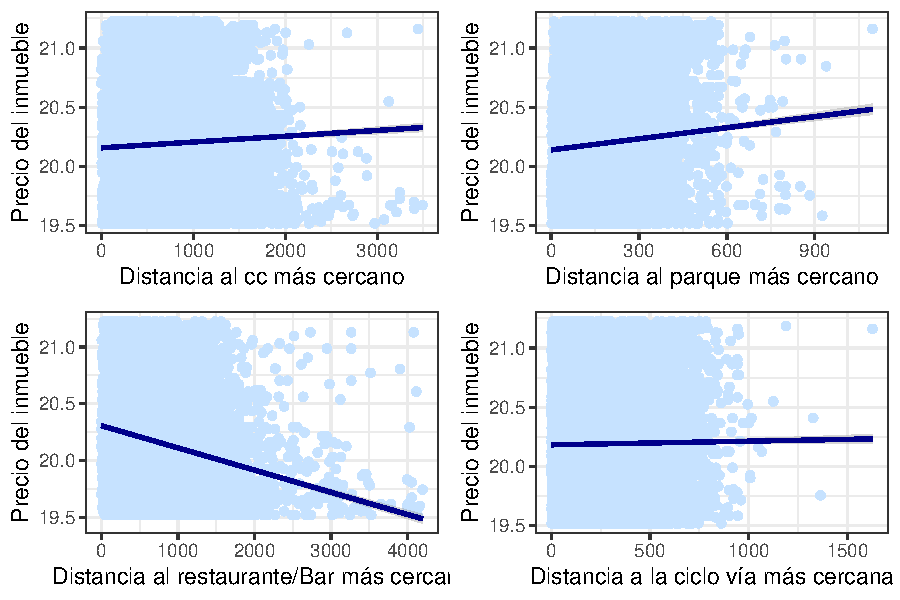
\includegraphics[width=0.8\textwidth]{graficos/scatter_conjunto.pdf}
             \label{fig:barras}
            \begin{minipage}{7\textwidth}
            \footnotesize
            \hspace{2cm} Fuente: Elaboración propia con train.csv, 2024.
            \end{minipage}
            \label{fig:scatters}
        \end{figure}


Como se puede observar en la figura \ref{fig:scatters}  para 1 de las 4 variables (específicamente para la distancia mínima a un restaurante o bar) existe una relación negativa con la variable de interés. Esto puede deberse a que los bares y restaurantes en Bogotá se encuentran altamente concentradas en ciertas zonas de la ciudad, por lo que las viviendas que se concentran en estas zonas pueden ser las de mayor precio\footnote{Hay que recalcar que estas zonas son las más concurridas tanto por locales como por turistas, por lo que es lógico pensar que son las zonas con los mayores precios de viviendas.}. Para las otras 3 variables se observa una relación positiva. Particularmente, se puede observar que hay una relación muy débil entre la variable de interés y la distancia a la ciclo ruta más cercana, esto puede sugerir que esta variable tiene bajo poder predictivo, lo que significaría alivianar el sesgo del modelo pero aumentar la varianza del modelo fuera de muestra.

\begin{figure}[H]
  \caption{Ubicacción de estaciones de trasporte en Bogota, D.C}\label{fig:hists}
  \hspace{-2cm} % Ajusta el espacio horizontal entre la figura y el margen izquierdo
  \subfloat[Ubicación de estaciones transmilenio\label{subfiga:Transmi}]{
    \includegraphics[width=0.7\textwidth, align=l]{graficos/mapatransmi.pdf}}
  \hspace{-2.8cm} % Ajusta el espacio horizontal entre las subfiguras
  \subfloat[Ubicación de estaciones de SITP\label{subfigb:sipt}]{
    \includegraphics[width=0.7\textwidth, align=l]{graficos/mapasitp.pdf}}
  \begin{center}
    \footnotesize{\textbf{Fuente:} Elaboración propia con train.csv, 2024.}
  \end{center}
\end{figure}


Ahora bien, el mapa de la izquierda (Figura \ref{subfiga:Transmi}) muestra las paradas del sistema de transporte masivo TransMilenio en Bogotá, con puntos rojos indicando las ubicaciones de estas paradas. Mientras que, el mapa de la derecha (Figura \ref{subfigb:sipt}) muestra las paradas del Sistema Integrado de Transporte Público (SITP) en Bogotá indicadas con puntos azules. Esta información es altamente relevante ya que la accesibilidad al transporte público es un factor importante que influye en los precios de las viviendas. Las propiedades cercanas a sistemas de transporte tienden a tener un valor más alto debido a la facilidad de desplazamiento. Además, si existe una alta cobertura del sistema de transporte, esta área suele estar mejor desarrollada en infraestructura y servicios. Ahora bien, observando el mapa izquierdo no existen muchas paradas de TransMilenio en la localidad de Chapinero, pero las que tiene tienen una gran conectividad con el Norte, Sur y Occidente de la ciudad. Además, reafirmando esta idea, el mapa de la derecha muestra una leve concentración de paradas de SITP en esta localidad, lo que intuye que los residentes de Chapinero pueden tener acceso a una red de transporte público eficiente y bien conectada, potencialmente aumentando el atractivo y valor de las propiedades en esta zona. \\

Es importante notar que la distribución de los puntos en el mapa revela una menor concentración de paradas de SITP en el norte de la ciudad en comparación con el centro y el sur. Además, las rutas de TransMilenio no cubren en su totalidad toda la ciudad. Existe una gran circulación de personas transitando por el centro de la ciudad, mientras que hacia las afueras la cantidad de personas disminuye notablemente. Esta desigual distribución puede influir en los precios de las viviendas, siendo más altas en las áreas mejor conectadas y desarrolladas.

\begin{table}[H]
\centering
\caption{Estadisticas de las posesiones}
\begin{tabular}{lrr}
\toprule
Variable & Sí & No \\
\midrule
Balcón & 8,541 & 22,776 \\
BBQ & 5,501 & 25,816 \\
Depósito & 12,654 & 18,663 \\
Ascensor & 6,197 & 25,120 \\
Patio & 3 & 31,314 \\
\bottomrule
\end{tabular}
\label{tab:posesiones} \\
\footnotesize Fuente: Elaboración propia con train.csv, 2024.

\end{table}


Por último, a partir de la cadena de caracteres que se tenía y manipuló inicialmente se pudo realizar la Tabla 2, la cual muestra algunas posesiones de los inmuebles en Bogotá; entre estos encontramos Barbecues, balones, depósitos, ascensores y por último patios. Si observamos esta última, podemos decir que son muy pocos los inmuebles que cuentan con patio, por lo que reafirmamos una vez más que nos encontramos con una base de datos con mayor concentración en apartamentos y no en casas, pues son estas que en el 99\% cuentan con un patio. Del resto de variables se puede observar que la mayoría de las observaciones no cuentan con estos “accesorios”.

\section{Analisis predictivo}

\subsection{Especificación de los modelos(variables)}

La especificación de los modelos involucraba alrededor de 75 variables tanto para el conjunto de datos de entrenamiento como para el conjunto de datos de testeo. Específicamente, se emplearon especificaciones de las variables de resultado en función de todos los predictores, sin incluir términos como variables al cuadrado o interacciones. Esta omisión se justificó por la utilización prevista de algoritmos como Boosting o redes neuronales, los cuales se espera que capturen las no linealidades de manera inherente. Este enfoque simplificado en la especificación de los modelos buscó facilitar la interpretación y el ajuste de los algoritmos, centrándose en la influencia directa de cada predictor en la variable de resultado. La especicifación de los modelos se puede resumir de la siguiente forma:

$$ln(price)=f(cuartos, area, distancia al CC mas cercano, hurtos cercanos, delitos sexuales cercanos, ..., etc)$$

\subsection{Resultados de los modelos}

A continuación la siguiente tabla presentara un resumen de los resultados de 6 modelos junto con el mejor modelo con mejor desempeño predictivo.

\begin{table}[H]
\centering
\caption{Punataje MAE de Kagle para diferentes modelos}
\begin{tabular}{ll}
\toprule
\textbf{Modelos} & \textbf{MAE de Kaggle} \\
\midrule
Regresión Lineal & 244.098.878,00 \\
Árbol de regresión & 229.238.184,00 \\
Random forest (mtry=42, min\_n=3) & 209.844.614,00 \\
Xgboosting (trees=500,min\_n=30,tree\_depth=6)& 185.475.938,00 \\
Redes neuronales  & 218.074.723,00 \\
Light gradient boosting (trees=600,min\_n=25,tree\_depth=4) & 184.662.023,00 \\
\textbf{Ensamble elastic net} \& \textbf{Light gradient boosting} & \textbf{183.535.559,00} \\
\bottomrule
\end{tabular} \\
\label{tab:mae_kaggle}
\footnotesize Fuente: Elaboración propia con train.csv, 2024.
\end{table}



Todos los modelos se entrenaron con la base de datos expuesta y el método de validación cruzada espacial con 5 submuestras. El modelo seleccionado tiene un MAE fuera de muestra de 183’500,000 COP, lo cual, a pesar de ser el valor más bajo de la métrica, representa un desfase absoluto medio significativo. Este modelo se estimó utilizando un método de ensamble mediante EN, donde los dos mejores modelos previamente estimados se combinaron para aumentar su poder predictivo. Se utilizaron dos modelos base para generar el ensamble, ambos de la familia de boosting. El primero fue estimado utilizando el algoritmo de lightgbm y el segundo utilizando extreme gradient boosting (xgb). Para la selección de hiper-parámetros de ambos modelos se buscó sobre la grilla completa de parámetros de manera iterativa, donde cada estimación buscaba reducir el MAE fuera de muestra.  \\

El proceso de optimización se inicializaba con una grilla amplia donde se le asignaba un rango razonable a cada hiper-parámetro. Si la estimación minimizaba el MAE eligiendo un parámetro en alguno de los límites de rango, se ampliaba este rango en la dirección indicada por el proceso de optimización. Si se elegía un parámetro interno al rango, se exploraban valores cercanos a este en la siguiente iteración. Si un mismo valor era elegido dos veces seguidas se elegia este valor como final para la optimización, es decir, en la siguiente estimación se dejaba fijo el hiper-parámetro elegido. Esto se hizo para ambos modelos hasta que se optimizaran todos los hiper-parámetros. \\

La tabla \ref{tab:mae_kaggle} se muestran los hiper-parámetros escogidos para lightgbm y XGB:
El mejor modelo de lightgbm según la métrica fuera de muestra (base de testeo) fue aquel que entrenaba 500 árboles, con una profundidad máxima de 6 niveles y un tamaño mínimo de nodos terminales de 30 observaciones. No se limitó la reducción de perdida (0), la tasa de aprendizaje se fijó en .05 y las variables escogidas al azar para generar un split fue de 45 variables. En el caso del XGB, el modelo que optimizo fuera de muestra fue aquel que entrenó 600 árboles, con una profundidad máxima de 4 niveles y un tamaño mínimo de nodos terminales de 25 observaciones. No se limitó la reducción de perdida (0) y siempre se entrenó sobre toda la muestra (sub-muestra = 1), la tasa de aprendizaje se fijó en .1 y las variables escogidas al azar para generar un split fue de 50 variables. \\

Después de entrenar los modelos optimizados sobre la totalidad de la muestra de entrenamiento se hicieron las predicciones de estos tanto en la muestra de entrenamiento como en la muestra de testeo, para posteriormente redondear estas predicciones al 100,000 COP más cercano (decidimos redondearlo así debido a que, si redondeábamos hacia abajo, la capacidad predictiva del modelo se reducía). Esto permite reducir los predictores de N a 2. Posteriormente, se creó una nueva base de entrenamiento que solo contaba con la variable de resultado (precio) y las predicciones de ambos modelos (en la de testeo solo contaba con los valores predichos). Sobre esta nueva base se estimó un modelo de elastic net utilizando validación cruzada estándar de 5 sub-muestras para optimizar los hiper-parámetros. Este proceso de optimización resultó en un modelo con ambos componentes (tanto lasso como ridge). Con el componente de lasso pesando .111 y el de ridge .0000000001. Utilizando este modelo y la base de testeo creada a partir de los métodos de boosting se hicieron las predicciones finales que posicionaron al equipo en el primer lugar de la competencia. \\

En términos de capacidad predictiva fuera de muestra, es decir, haciendo referencia a la métrica (MAE) calculada por la plataforma Kaggle a partir de las predicciones hechas sobre la base de testeo, el modelo de ensamblaje de lightgbm y XGB mediante elastic net es el más preciso con un MAE de 183’500,000 COP. El segundo mejor modelo según esta metrica fue el estimado mediante lightgbm utilizando los hiper-parámetros y métodos de muestreo y redondeo previamente discutidos. Sus predicciones fueron, en promedio, 1’800,000 COP menos precisas que el ensamble en términos absolutos. El tercer modelo fue el XGB con los hiper-parametros, técnicas de re-muestreo y redondeo previamente expuestas, generando predicciones que, en promedio, eran 1’900,000 COP menos precisas que el ensamble en términos absolutos. Finalmente, el random forest con 3 observaciones en cada nodo y 42 predictores, a través de las técnicas de Re-muestreo utilizadas en los otros modelos se encontró que es, en promedio, 26’300,000 COP menos preciso que el modelo de ensamblaje en términos absolutos.

\subsection{Análisis de sesgo predictivo y sobre-ajuste}


Con el objetivo de determinar si el modelo tendía a sobreestimar o subestimar las predicciones, se llevó a cabo un análisis de validación cruzada, dado que no se cuenta con la información de los precios del conjunto de datos de prueba. Se calculó el porcentaje de ocasiones en las que el modelo ajustaba por encima del precio real de la propiedad para cada uno de los cinco splits de la validación cruzada espacial. Los resultados se presentan en la siguiente tabla, donde se detalla la frecuencia relativa con la que el modelo superaba el valor real de la propiedad en cada conjunto de datos geográficamente separados. Estos hallazgos proporcionan una visión crítica sobre el desempeño del modelo en términos de su capacidad para predecir con precisión los valores inmobiliarios.

\begin{table}[H]
\centering
\caption{Frecuencia con la que el modelo predijo valores por encima del precio real y MAE}
\begin{tabular}{@{\extracolsep{5pt}}lcc}
\\[-1.8ex]\hline
\hline \\[-1.8ex]
Test Split & $Price-\hat{price} \geq 0$& MAE \\
\hline \\[-1.8ex]
1 & 43\% & \$76,333,554.00 \\
2 & 43\% & \$91,938,174.00 \\
3 & 44\% & \$100,568,199.00 \\
4 & 41\% & \$95,375,916.00 \\
5 & 42\% & \$105,729,926.00 \\
\hline \\[-1.8ex]
\end{tabular}

\label{tab:sobreajuste}
\footnotesize Fuente: Elaboración propia con train.csv, 2024.
\end{table}


Como se puede apreciar en la tabla anterior, en todos los test splits del k-fold cross validation con k=5, se evidenció que el modelo siempre predice una cantidad menor de valores por encima del precio real. Esto implica que el modelo tiende a estimar más valores por debajo del precio real, sugiriendo que el mejor modelo tiende a subestimar los precios de las viviendas, lo cual se considera una desventaja significativa, especialmente considerando que el error promedio de valoración es de 183 millones de COP fuera de muestra. No obstante, este análisis representa solo un acercamiento al posible comportamiento fuera de muestra del modelo, realizado debido a la ausencia de precios en el conjunto de datos de prueba. \\

Por otro lado, la tabla \ref{tab:sobreajuste} también presente el MAE  de los splits de prueba de prueba de la validación cruzada. Como se puede notar este MAE difiere de forma considerable en comparación con el MAE  de la tabla  \ref{tab:mae_kaggle}. Aproximadamente la diferencia entre los puntajes entre el mejor modelo y los puntajes de la tabla \ref{tab:sobreajuste} esta entre  80 millones de COP y 110 millones de COP. Considerando que el MAE de los splits de prueba de la validación de cruzada siempre esta significativamente por debajo se puede afirmar que el mejor modelo de predicción en Kagle sufre de sobresajuste. Esto se considera una debilidad a tener en cuenta por parte de los modelos estimados a traves del algoritmo que arrojo mejores resultados debido a que el modelo no tiene la capacidad de estimar predicciones de calidad fuera de muestra pero si cuenta con la capacidad de realizar predicciones dentro de la muestra.

\section{Conclusión y recomendaciones}

Para finalizar, se concluye que un error de predicción de 183 millones de COP fuera de muestra plantea serias dudas sobre la confiabilidad de los resultados de los algoritmos de machine learning presentados. Un margen de error tan considerable dificulta la fiabilidad de los modelos, lo que hace que sea prácticamente imposible encontrar oportunidades de negocio en las que el modelo valore adecuadamente las propiedades para comprarlas por debajo de su precio de mercado. Esta falta de confiabilidad pone en entredicho la utilidad práctica de los modelos en el contexto de la valoración de bienes raíces. \\

Se recomienda encarecidamente explorar diferentes enfoques para el manejo de datos con el objetivo de reducir el Error Medio Absoluto. Este puede incluir la incorporación de más variables relevantes, la eliminación de datos mas atípicos que puedan estar inflando o subestimando el error. Al mejorar la calidad y la representatividad de los datos de entrada, es posible que se logre una mejora significativa en la precisión de las predicciones del modelo. \\

Además, se sugiere explorar la utilización de una variedad diferente de algoritmos presentados en el documento con el fin de mitigar el sobreajuste del modelo. Esto puede implicar probar modelos más simples o complejos, ajustar los hiperparámetros de manera más cuidadosa o implementar técnicas de regularización mejores para evitar que el modelo se ajuste demasiado a los datos de entrenamiento. Asimismo, se recomienda el uso de métricas que penalizen más las predicciones por encima del precio real, lo que fomentaría un escenario donde el modelo sea más propenso a predecir adecuadamente los precios. De esta manera, cuando el algoritmo presente una predicción por encima del precio real, se pueda interpretar como una oportunidad de negocio, ya que indicaría la posibilidad de adquirir una propiedad por debajo de su valor potencial en el mercado.

\section*{Referencias}

\begin{itemize}
    \item[$\bullet$] DANE. (2024). Comunicado de prensa. Recuperado de https://www.dane.gov.co/files/operaciones/PIB/cp-PIB-Itrim2024.pdf
    \item[$\bullet$]  Knauff, J. (2021). Cómo el cierre de Zillow de su división Home-Flipping causará daños a la marca a largo plazo. Entrepreneur. https://www.entrepreneur.com/es/noticias/como-el-cierre-de-zillow-de-su-division-home-flipping/409372
\end{itemize}






\end{document}